% Created by tikzDevice version 0.12.6 on 2025-08-19 18:36:04
% !TEX encoding = UTF-8 Unicode
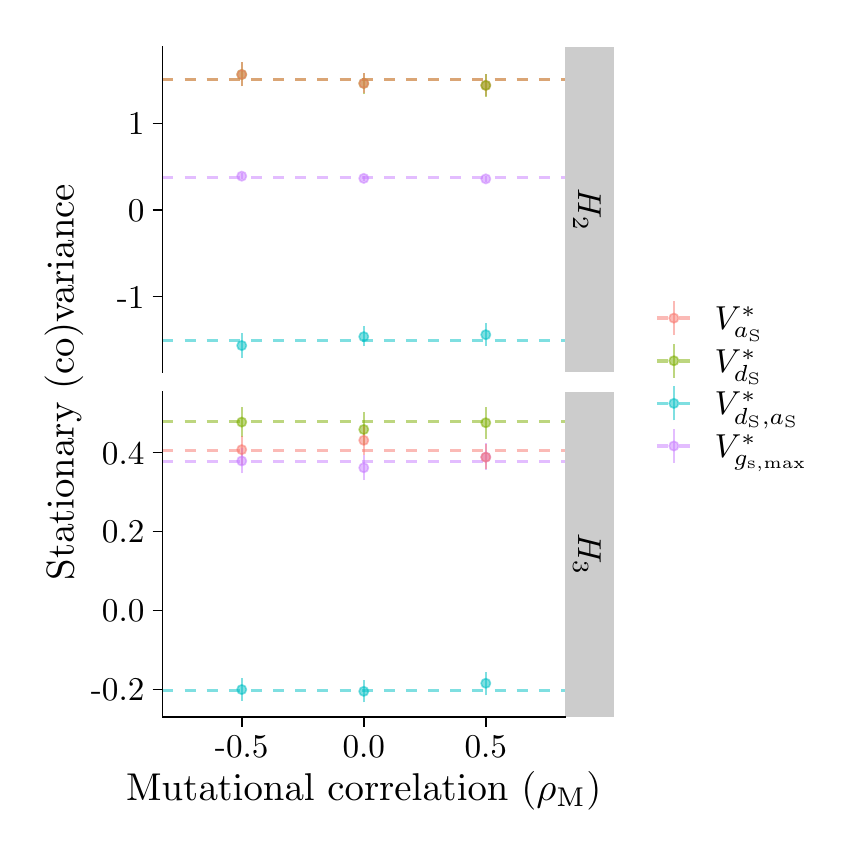
\begin{tikzpicture}[x=1pt,y=1pt]
\definecolor{fillColor}{RGB}{255,255,255}
\path[use as bounding box,fill=fillColor,fill opacity=0.00] (0,0) rectangle (289.08,289.08);
\begin{scope}
\path[clip] ( 48.69,164.52) rectangle (194.20,282.08);
\definecolor{drawColor}{RGB}{124,174,0}

\path[draw=drawColor,draw opacity=0.50,line width= 1.3pt,dash pattern=on 4pt off 4pt ,line join=round] ( 48.69,270.39) -- (194.20,270.39);
\definecolor{drawColor}{RGB}{248,118,109}

\path[draw=drawColor,draw opacity=0.50,line width= 1.3pt,dash pattern=on 4pt off 4pt ,line join=round] ( 48.69,270.39) -- (194.20,270.39);
\definecolor{drawColor}{RGB}{0,191,196}

\path[draw=drawColor,draw opacity=0.50,line width= 1.3pt,dash pattern=on 4pt off 4pt ,line join=round] ( 48.69,175.98) -- (194.20,175.98);
\definecolor{drawColor}{RGB}{199,124,255}

\path[draw=drawColor,draw opacity=0.50,line width= 1.3pt,dash pattern=on 4pt off 4pt ,line join=round] ( 48.69,234.98) -- (194.20,234.98);
\definecolor{drawColor}{RGB}{0,191,196}

\path[draw=drawColor,draw opacity=0.50,line width= 0.7pt,line join=round] ( 77.35,169.86) -- ( 77.35,178.75);
\definecolor{drawColor}{RGB}{124,174,0}

\path[draw=drawColor,draw opacity=0.50,line width= 0.7pt,line join=round] ( 77.35,267.87) -- ( 77.35,276.67);
\definecolor{drawColor}{RGB}{248,118,109}

\path[draw=drawColor,draw opacity=0.50,line width= 0.7pt,line join=round] ( 77.35,267.99) -- ( 77.35,276.74);
\definecolor{drawColor}{RGB}{0,191,196}

\path[draw=drawColor,draw opacity=0.50,line width= 0.7pt,line join=round] (165.54,174.04) -- (165.54,182.46);
\definecolor{drawColor}{RGB}{248,118,109}

\path[draw=drawColor,draw opacity=0.50,line width= 0.7pt,line join=round] (165.54,264.25) -- (165.54,272.45);
\definecolor{drawColor}{RGB}{124,174,0}

\path[draw=drawColor,draw opacity=0.50,line width= 0.7pt,line join=round] (165.54,264.16) -- (165.54,272.18);

\path[draw=drawColor,draw opacity=0.50,line width= 0.7pt,line join=round] (121.45,264.99) -- (121.45,272.62);
\definecolor{drawColor}{RGB}{248,118,109}

\path[draw=drawColor,draw opacity=0.50,line width= 0.7pt,line join=round] (121.45,265.31) -- (121.45,272.62);
\definecolor{drawColor}{RGB}{0,191,196}

\path[draw=drawColor,draw opacity=0.50,line width= 0.7pt,line join=round] (121.45,173.93) -- (121.45,181.20);
\definecolor{drawColor}{RGB}{199,124,255}

\path[draw=drawColor,draw opacity=0.50,line width= 0.7pt,line join=round] ( 77.35,234.35) -- ( 77.35,236.51);

\path[draw=drawColor,draw opacity=0.50,line width= 0.7pt,line join=round] (165.54,233.47) -- (165.54,235.47);

\path[draw=drawColor,draw opacity=0.50,line width= 0.7pt,line join=round] (121.45,233.71) -- (121.45,235.50);
\definecolor{drawColor}{RGB}{0,191,196}
\definecolor{fillColor}{RGB}{0,191,196}

\path[draw=drawColor,draw opacity=0.50,line width= 0.6pt,line join=round,line cap=round,fill=fillColor,fill opacity=0.50] ( 77.35,174.21) circle (  1.69);
\definecolor{drawColor}{RGB}{124,174,0}
\definecolor{fillColor}{RGB}{124,174,0}

\path[draw=drawColor,draw opacity=0.50,line width= 0.6pt,line join=round,line cap=round,fill=fillColor,fill opacity=0.50] ( 77.35,272.15) circle (  1.69);
\definecolor{drawColor}{RGB}{248,118,109}
\definecolor{fillColor}{RGB}{248,118,109}

\path[draw=drawColor,draw opacity=0.50,line width= 0.6pt,line join=round,line cap=round,fill=fillColor,fill opacity=0.50] ( 77.35,272.16) circle (  1.69);
\definecolor{drawColor}{RGB}{0,191,196}
\definecolor{fillColor}{RGB}{0,191,196}

\path[draw=drawColor,draw opacity=0.50,line width= 0.6pt,line join=round,line cap=round,fill=fillColor,fill opacity=0.50] (165.54,178.14) circle (  1.69);
\definecolor{drawColor}{RGB}{248,118,109}
\definecolor{fillColor}{RGB}{248,118,109}

\path[draw=drawColor,draw opacity=0.50,line width= 0.6pt,line join=round,line cap=round,fill=fillColor,fill opacity=0.50] (165.54,268.24) circle (  1.69);
\definecolor{drawColor}{RGB}{124,174,0}
\definecolor{fillColor}{RGB}{124,174,0}

\path[draw=drawColor,draw opacity=0.50,line width= 0.6pt,line join=round,line cap=round,fill=fillColor,fill opacity=0.50] (165.54,268.22) circle (  1.69);

\path[draw=drawColor,draw opacity=0.50,line width= 0.6pt,line join=round,line cap=round,fill=fillColor,fill opacity=0.50] (121.45,268.94) circle (  1.69);
\definecolor{drawColor}{RGB}{248,118,109}
\definecolor{fillColor}{RGB}{248,118,109}

\path[draw=drawColor,draw opacity=0.50,line width= 0.6pt,line join=round,line cap=round,fill=fillColor,fill opacity=0.50] (121.45,268.95) circle (  1.69);
\definecolor{drawColor}{RGB}{0,191,196}
\definecolor{fillColor}{RGB}{0,191,196}

\path[draw=drawColor,draw opacity=0.50,line width= 0.6pt,line join=round,line cap=round,fill=fillColor,fill opacity=0.50] (121.45,177.42) circle (  1.69);
\definecolor{drawColor}{RGB}{199,124,255}
\definecolor{fillColor}{RGB}{199,124,255}

\path[draw=drawColor,draw opacity=0.50,line width= 0.6pt,line join=round,line cap=round,fill=fillColor,fill opacity=0.50] ( 77.35,235.42) circle (  1.69);

\path[draw=drawColor,draw opacity=0.50,line width= 0.6pt,line join=round,line cap=round,fill=fillColor,fill opacity=0.50] (165.54,234.44) circle (  1.69);

\path[draw=drawColor,draw opacity=0.50,line width= 0.6pt,line join=round,line cap=round,fill=fillColor,fill opacity=0.50] (121.45,234.62) circle (  1.69);
\end{scope}
\begin{scope}
\path[clip] ( 48.69, 39.96) rectangle (194.20,157.52);
\definecolor{drawColor}{RGB}{124,174,0}

\path[draw=drawColor,draw opacity=0.50,line width= 1.3pt,dash pattern=on 4pt off 4pt ,line join=round] ( 48.69,146.73) -- (194.20,146.73);
\definecolor{drawColor}{RGB}{248,118,109}

\path[draw=drawColor,draw opacity=0.50,line width= 1.3pt,dash pattern=on 4pt off 4pt ,line join=round] ( 48.69,136.22) -- (194.20,136.22);
\definecolor{drawColor}{RGB}{0,191,196}

\path[draw=drawColor,draw opacity=0.50,line width= 1.3pt,dash pattern=on 4pt off 4pt ,line join=round] ( 48.69, 49.61) -- (194.20, 49.61);
\definecolor{drawColor}{RGB}{199,124,255}

\path[draw=drawColor,draw opacity=0.50,line width= 1.3pt,dash pattern=on 4pt off 4pt ,line join=round] ( 48.69,132.29) -- (194.20,132.29);
\definecolor{drawColor}{RGB}{124,174,0}

\path[draw=drawColor,draw opacity=0.50,line width= 0.7pt,line join=round] (121.45,138.34) -- (121.45,150.22);

\path[draw=drawColor,draw opacity=0.50,line width= 0.7pt,line join=round] (165.54,140.39) -- (165.54,151.95);

\path[draw=drawColor,draw opacity=0.50,line width= 0.7pt,line join=round] ( 77.35,141.33) -- ( 77.35,152.18);
\definecolor{drawColor}{RGB}{248,118,109}

\path[draw=drawColor,draw opacity=0.50,line width= 0.7pt,line join=round] ( 77.35,131.12) -- ( 77.35,141.65);

\path[draw=drawColor,draw opacity=0.50,line width= 0.7pt,line join=round] (121.45,134.82) -- (121.45,145.18);
\definecolor{drawColor}{RGB}{199,124,255}

\path[draw=drawColor,draw opacity=0.50,line width= 0.7pt,line join=round] (165.54,129.21) -- (165.54,138.93);

\path[draw=drawColor,draw opacity=0.50,line width= 0.7pt,line join=round] ( 77.35,127.98) -- ( 77.35,137.20);
\definecolor{drawColor}{RGB}{248,118,109}

\path[draw=drawColor,draw opacity=0.50,line width= 0.7pt,line join=round] (165.54,129.49) -- (165.54,138.67);
\definecolor{drawColor}{RGB}{199,124,255}

\path[draw=drawColor,draw opacity=0.50,line width= 0.7pt,line join=round] (121.45,125.57) -- (121.45,134.61);
\definecolor{drawColor}{RGB}{0,191,196}

\path[draw=drawColor,draw opacity=0.50,line width= 0.7pt,line join=round] (165.54, 47.82) -- (165.54, 56.43);

\path[draw=drawColor,draw opacity=0.50,line width= 0.7pt,line join=round] ( 77.35, 45.86) -- ( 77.35, 53.98);

\path[draw=drawColor,draw opacity=0.50,line width= 0.7pt,line join=round] (121.45, 45.30) -- (121.45, 53.22);
\definecolor{drawColor}{RGB}{124,174,0}
\definecolor{fillColor}{RGB}{124,174,0}

\path[draw=drawColor,draw opacity=0.50,line width= 0.6pt,line join=round,line cap=round,fill=fillColor,fill opacity=0.50] (121.45,143.89) circle (  1.69);

\path[draw=drawColor,draw opacity=0.50,line width= 0.6pt,line join=round,line cap=round,fill=fillColor,fill opacity=0.50] (165.54,146.32) circle (  1.69);

\path[draw=drawColor,draw opacity=0.50,line width= 0.6pt,line join=round,line cap=round,fill=fillColor,fill opacity=0.50] ( 77.35,146.55) circle (  1.69);
\definecolor{drawColor}{RGB}{248,118,109}
\definecolor{fillColor}{RGB}{248,118,109}

\path[draw=drawColor,draw opacity=0.50,line width= 0.6pt,line join=round,line cap=round,fill=fillColor,fill opacity=0.50] ( 77.35,136.60) circle (  1.69);

\path[draw=drawColor,draw opacity=0.50,line width= 0.6pt,line join=round,line cap=round,fill=fillColor,fill opacity=0.50] (121.45,139.97) circle (  1.69);
\definecolor{drawColor}{RGB}{199,124,255}
\definecolor{fillColor}{RGB}{199,124,255}

\path[draw=drawColor,draw opacity=0.50,line width= 0.6pt,line join=round,line cap=round,fill=fillColor,fill opacity=0.50] (165.54,133.88) circle (  1.69);

\path[draw=drawColor,draw opacity=0.50,line width= 0.6pt,line join=round,line cap=round,fill=fillColor,fill opacity=0.50] ( 77.35,132.51) circle (  1.69);
\definecolor{drawColor}{RGB}{248,118,109}
\definecolor{fillColor}{RGB}{248,118,109}

\path[draw=drawColor,draw opacity=0.50,line width= 0.6pt,line join=round,line cap=round,fill=fillColor,fill opacity=0.50] (165.54,133.88) circle (  1.69);
\definecolor{drawColor}{RGB}{199,124,255}
\definecolor{fillColor}{RGB}{199,124,255}

\path[draw=drawColor,draw opacity=0.50,line width= 0.6pt,line join=round,line cap=round,fill=fillColor,fill opacity=0.50] (121.45,130.06) circle (  1.69);
\definecolor{drawColor}{RGB}{0,191,196}
\definecolor{fillColor}{RGB}{0,191,196}

\path[draw=drawColor,draw opacity=0.50,line width= 0.6pt,line join=round,line cap=round,fill=fillColor,fill opacity=0.50] (165.54, 52.18) circle (  1.69);

\path[draw=drawColor,draw opacity=0.50,line width= 0.6pt,line join=round,line cap=round,fill=fillColor,fill opacity=0.50] ( 77.35, 49.91) circle (  1.69);

\path[draw=drawColor,draw opacity=0.50,line width= 0.6pt,line join=round,line cap=round,fill=fillColor,fill opacity=0.50] (121.45, 49.27) circle (  1.69);
\end{scope}
\begin{scope}
\path[clip] (194.20,164.52) rectangle (211.80,282.08);
\definecolor{fillColor}{gray}{0.80}

\path[fill=fillColor] (194.20,164.52) rectangle (211.80,282.08);
\definecolor{drawColor}{RGB}{0,0,0}

\node[text=drawColor,rotate=-90.00,anchor=base,inner sep=0pt, outer sep=0pt, scale=  1.20] at (198.87,223.30) {$H_2$};
\end{scope}
\begin{scope}
\path[clip] (194.20, 39.96) rectangle (211.80,157.52);
\definecolor{fillColor}{gray}{0.80}

\path[fill=fillColor] (194.20, 39.96) rectangle (211.80,157.52);
\definecolor{drawColor}{RGB}{0,0,0}

\node[text=drawColor,rotate=-90.00,anchor=base,inner sep=0pt, outer sep=0pt, scale=  1.20] at (198.87, 98.74) {$H_3$};
\end{scope}
\begin{scope}
\path[clip] (  0.00,  0.00) rectangle (289.08,289.08);
\definecolor{drawColor}{RGB}{0,0,0}

\path[draw=drawColor,line width= 0.6pt,line join=round,line cap=rect] ( 48.69, 39.96) --
	(194.20, 39.96);
\end{scope}
\begin{scope}
\path[clip] (  0.00,  0.00) rectangle (289.08,289.08);
\definecolor{drawColor}{RGB}{0,0,0}

\path[draw=drawColor,line width= 0.6pt,line join=round] ( 77.35, 36.46) --
	( 77.35, 39.96);

\path[draw=drawColor,line width= 0.6pt,line join=round] (121.45, 36.46) --
	(121.45, 39.96);

\path[draw=drawColor,line width= 0.6pt,line join=round] (165.54, 36.46) --
	(165.54, 39.96);
\end{scope}
\begin{scope}
\path[clip] (  0.00,  0.00) rectangle (289.08,289.08);
\definecolor{drawColor}{RGB}{0,0,0}

\node[text=drawColor,anchor=base,inner sep=0pt, outer sep=0pt, scale=  1.20] at ( 77.35, 25.20) {-0.5};

\node[text=drawColor,anchor=base,inner sep=0pt, outer sep=0pt, scale=  1.20] at (121.45, 25.20) {0.0};

\node[text=drawColor,anchor=base,inner sep=0pt, outer sep=0pt, scale=  1.20] at (165.54, 25.20) {0.5};
\end{scope}
\begin{scope}
\path[clip] (  0.00,  0.00) rectangle (289.08,289.08);
\definecolor{drawColor}{RGB}{0,0,0}

\path[draw=drawColor,line width= 0.6pt,line join=round,line cap=rect] ( 48.69,164.52) --
	( 48.69,282.08);
\end{scope}
\begin{scope}
\path[clip] (  0.00,  0.00) rectangle (289.08,289.08);
\definecolor{drawColor}{RGB}{0,0,0}

\node[text=drawColor,anchor=base east,inner sep=0pt, outer sep=0pt, scale=  1.20] at ( 42.19,187.77) {-1};

\node[text=drawColor,anchor=base east,inner sep=0pt, outer sep=0pt, scale=  1.20] at ( 42.19,219.05) {0};

\node[text=drawColor,anchor=base east,inner sep=0pt, outer sep=0pt, scale=  1.20] at ( 42.19,250.33) {1};
\end{scope}
\begin{scope}
\path[clip] (  0.00,  0.00) rectangle (289.08,289.08);
\definecolor{drawColor}{RGB}{0,0,0}

\path[draw=drawColor,line width= 0.6pt,line join=round] ( 45.19,191.90) --
	( 48.69,191.90);

\path[draw=drawColor,line width= 0.6pt,line join=round] ( 45.19,223.18) --
	( 48.69,223.18);

\path[draw=drawColor,line width= 0.6pt,line join=round] ( 45.19,254.46) --
	( 48.69,254.46);
\end{scope}
\begin{scope}
\path[clip] (  0.00,  0.00) rectangle (289.08,289.08);
\definecolor{drawColor}{RGB}{0,0,0}

\path[draw=drawColor,line width= 0.6pt,line join=round,line cap=rect] ( 48.69, 39.96) --
	( 48.69,157.52);
\end{scope}
\begin{scope}
\path[clip] (  0.00,  0.00) rectangle (289.08,289.08);
\definecolor{drawColor}{RGB}{0,0,0}

\node[text=drawColor,anchor=base east,inner sep=0pt, outer sep=0pt, scale=  1.20] at ( 42.19, 45.82) {-0.2};

\node[text=drawColor,anchor=base east,inner sep=0pt, outer sep=0pt, scale=  1.20] at ( 42.19, 74.35) {0.0};

\node[text=drawColor,anchor=base east,inner sep=0pt, outer sep=0pt, scale=  1.20] at ( 42.19,102.87) {0.2};

\node[text=drawColor,anchor=base east,inner sep=0pt, outer sep=0pt, scale=  1.20] at ( 42.19,131.40) {0.4};
\end{scope}
\begin{scope}
\path[clip] (  0.00,  0.00) rectangle (289.08,289.08);
\definecolor{drawColor}{RGB}{0,0,0}

\path[draw=drawColor,line width= 0.6pt,line join=round] ( 45.19, 49.95) --
	( 48.69, 49.95);

\path[draw=drawColor,line width= 0.6pt,line join=round] ( 45.19, 78.48) --
	( 48.69, 78.48);

\path[draw=drawColor,line width= 0.6pt,line join=round] ( 45.19,107.00) --
	( 48.69,107.00);

\path[draw=drawColor,line width= 0.6pt,line join=round] ( 45.19,135.53) --
	( 48.69,135.53);
\end{scope}
\begin{scope}
\path[clip] (  0.00,  0.00) rectangle (289.08,289.08);
\definecolor{drawColor}{RGB}{0,0,0}

\node[text=drawColor,anchor=base,inner sep=0pt, outer sep=0pt, scale=  1.40] at (121.45,  9.72) {Mutational correlation ($\rho_\mathrm{M}$)};
\end{scope}
\begin{scope}
\path[clip] (  0.00,  0.00) rectangle (289.08,289.08);
\definecolor{drawColor}{RGB}{0,0,0}

\node[text=drawColor,rotate= 90.00,anchor=base,inner sep=0pt, outer sep=0pt, scale=  1.40] at ( 16.64,161.02) {Stationary (co)variance};
\end{scope}
\begin{scope}
\path[clip] (  0.00,  0.00) rectangle (289.08,289.08);
\definecolor{drawColor}{RGB}{248,118,109}

\path[draw=drawColor,draw opacity=0.50,line width= 1.3pt,dash pattern=on 4pt off 4pt ,line join=round] (227.34,184.12) -- (239.66,184.12);
\end{scope}
\begin{scope}
\path[clip] (  0.00,  0.00) rectangle (289.08,289.08);
\definecolor{drawColor}{RGB}{248,118,109}

\path[draw=drawColor,draw opacity=0.50,line width= 0.7pt,line join=round] (233.50,177.96) -- (233.50,190.28);
\definecolor{fillColor}{RGB}{248,118,109}

\path[draw=drawColor,draw opacity=0.50,line width= 0.6pt,line join=round,line cap=round,fill=fillColor,fill opacity=0.50] (233.50,184.12) circle (  1.69);
\end{scope}
\begin{scope}
\path[clip] (  0.00,  0.00) rectangle (289.08,289.08);
\definecolor{drawColor}{RGB}{124,174,0}

\path[draw=drawColor,draw opacity=0.50,line width= 1.3pt,dash pattern=on 4pt off 4pt ,line join=round] (227.34,168.72) -- (239.66,168.72);
\end{scope}
\begin{scope}
\path[clip] (  0.00,  0.00) rectangle (289.08,289.08);
\definecolor{drawColor}{RGB}{124,174,0}

\path[draw=drawColor,draw opacity=0.50,line width= 0.7pt,line join=round] (233.50,162.56) -- (233.50,174.88);
\definecolor{fillColor}{RGB}{124,174,0}

\path[draw=drawColor,draw opacity=0.50,line width= 0.6pt,line join=round,line cap=round,fill=fillColor,fill opacity=0.50] (233.50,168.72) circle (  1.69);
\end{scope}
\begin{scope}
\path[clip] (  0.00,  0.00) rectangle (289.08,289.08);
\definecolor{drawColor}{RGB}{0,191,196}

\path[draw=drawColor,draw opacity=0.50,line width= 1.3pt,dash pattern=on 4pt off 4pt ,line join=round] (227.34,153.32) -- (239.66,153.32);
\end{scope}
\begin{scope}
\path[clip] (  0.00,  0.00) rectangle (289.08,289.08);
\definecolor{drawColor}{RGB}{0,191,196}

\path[draw=drawColor,draw opacity=0.50,line width= 0.7pt,line join=round] (233.50,147.16) -- (233.50,159.48);
\definecolor{fillColor}{RGB}{0,191,196}

\path[draw=drawColor,draw opacity=0.50,line width= 0.6pt,line join=round,line cap=round,fill=fillColor,fill opacity=0.50] (233.50,153.32) circle (  1.69);
\end{scope}
\begin{scope}
\path[clip] (  0.00,  0.00) rectangle (289.08,289.08);
\definecolor{drawColor}{RGB}{199,124,255}

\path[draw=drawColor,draw opacity=0.50,line width= 1.3pt,dash pattern=on 4pt off 4pt ,line join=round] (227.34,137.92) -- (239.66,137.92);
\end{scope}
\begin{scope}
\path[clip] (  0.00,  0.00) rectangle (289.08,289.08);
\definecolor{drawColor}{RGB}{199,124,255}

\path[draw=drawColor,draw opacity=0.50,line width= 0.7pt,line join=round] (233.50,131.76) -- (233.50,144.08);
\definecolor{fillColor}{RGB}{199,124,255}

\path[draw=drawColor,draw opacity=0.50,line width= 0.6pt,line join=round,line cap=round,fill=fillColor,fill opacity=0.50] (233.50,137.92) circle (  1.69);
\end{scope}
\begin{scope}
\path[clip] (  0.00,  0.00) rectangle (289.08,289.08);
\definecolor{drawColor}{RGB}{0,0,0}

\node[text=drawColor,anchor=base west,inner sep=0pt, outer sep=0pt, scale=  1.20] at (248.20,179.99) {$V^*_{a_\mathrm{S}}$};
\end{scope}
\begin{scope}
\path[clip] (  0.00,  0.00) rectangle (289.08,289.08);
\definecolor{drawColor}{RGB}{0,0,0}

\node[text=drawColor,anchor=base west,inner sep=0pt, outer sep=0pt, scale=  1.20] at (248.20,164.59) {$V^*_{d_\mathrm{S}}$};
\end{scope}
\begin{scope}
\path[clip] (  0.00,  0.00) rectangle (289.08,289.08);
\definecolor{drawColor}{RGB}{0,0,0}

\node[text=drawColor,anchor=base west,inner sep=0pt, outer sep=0pt, scale=  1.20] at (248.20,149.19) {$V^*_{d_\mathrm{S},a_\mathrm{S}}$};
\end{scope}
\begin{scope}
\path[clip] (  0.00,  0.00) rectangle (289.08,289.08);
\definecolor{drawColor}{RGB}{0,0,0}

\node[text=drawColor,anchor=base west,inner sep=0pt, outer sep=0pt, scale=  1.20] at (248.20,133.79) {$V^*_{g_\mathrm{s,max}}$};
\end{scope}
\end{tikzpicture}
